%=====================================================================
\section{Monday 5 October: flow, wall lattice dynamics, edge criteria}\label{sec:monday}

\subsection{Flow and wall-defect tilt in circles}
Per-frame flow reduction of 930 circle runs ($\rho\le0.15$, $\pm k$, 3 seeds) on the server (Fig.~\ref{fig:flow}).
\begin{itemize}
  \item The mean azimuthal flow $|\langle v_\theta\rangle|$ collapses on $R/\la$ for all $\rho$: $\approx0.35$ at $0.6\,\la$,
        0.9--1.0 at 2--2.5\,$\la$ (Mach $\sim1$). The circulation fraction is 0.8--0.9 between 0.5 and $2.5\,\la$; for $+k$
        it collapses to 0.2--0.4 (reversals) above $\approx2.5\,\la$, the same size where the layer is lost. No coherent
        vortex below $0.4\,\la$.
  \item Enstrophy peaks ($\approx0.01$--0.015) at $R\approx0.4$--$0.5\,\la$ and decays to 0.004 at $2.9\,\la$; $+k$ exceeds
        $-k$ by 20--30\% below $2\,\la$.
  \item Wall $+\tfrac12$ lean downstream by 60--65$^\circ$ at $\rho\le0.06$, 30--40$^\circ$ at $\rho=0.14$--0.15; the tilt
        vanishes where the layer is lost. Wall $-\tfrac12$ lean downstream by 8--15$^\circ$. The tilt sign agrees with the
        circulation in $\approx100\%$ of frames inside the layer window.
\end{itemize}
\begin{figure}[h]\centering
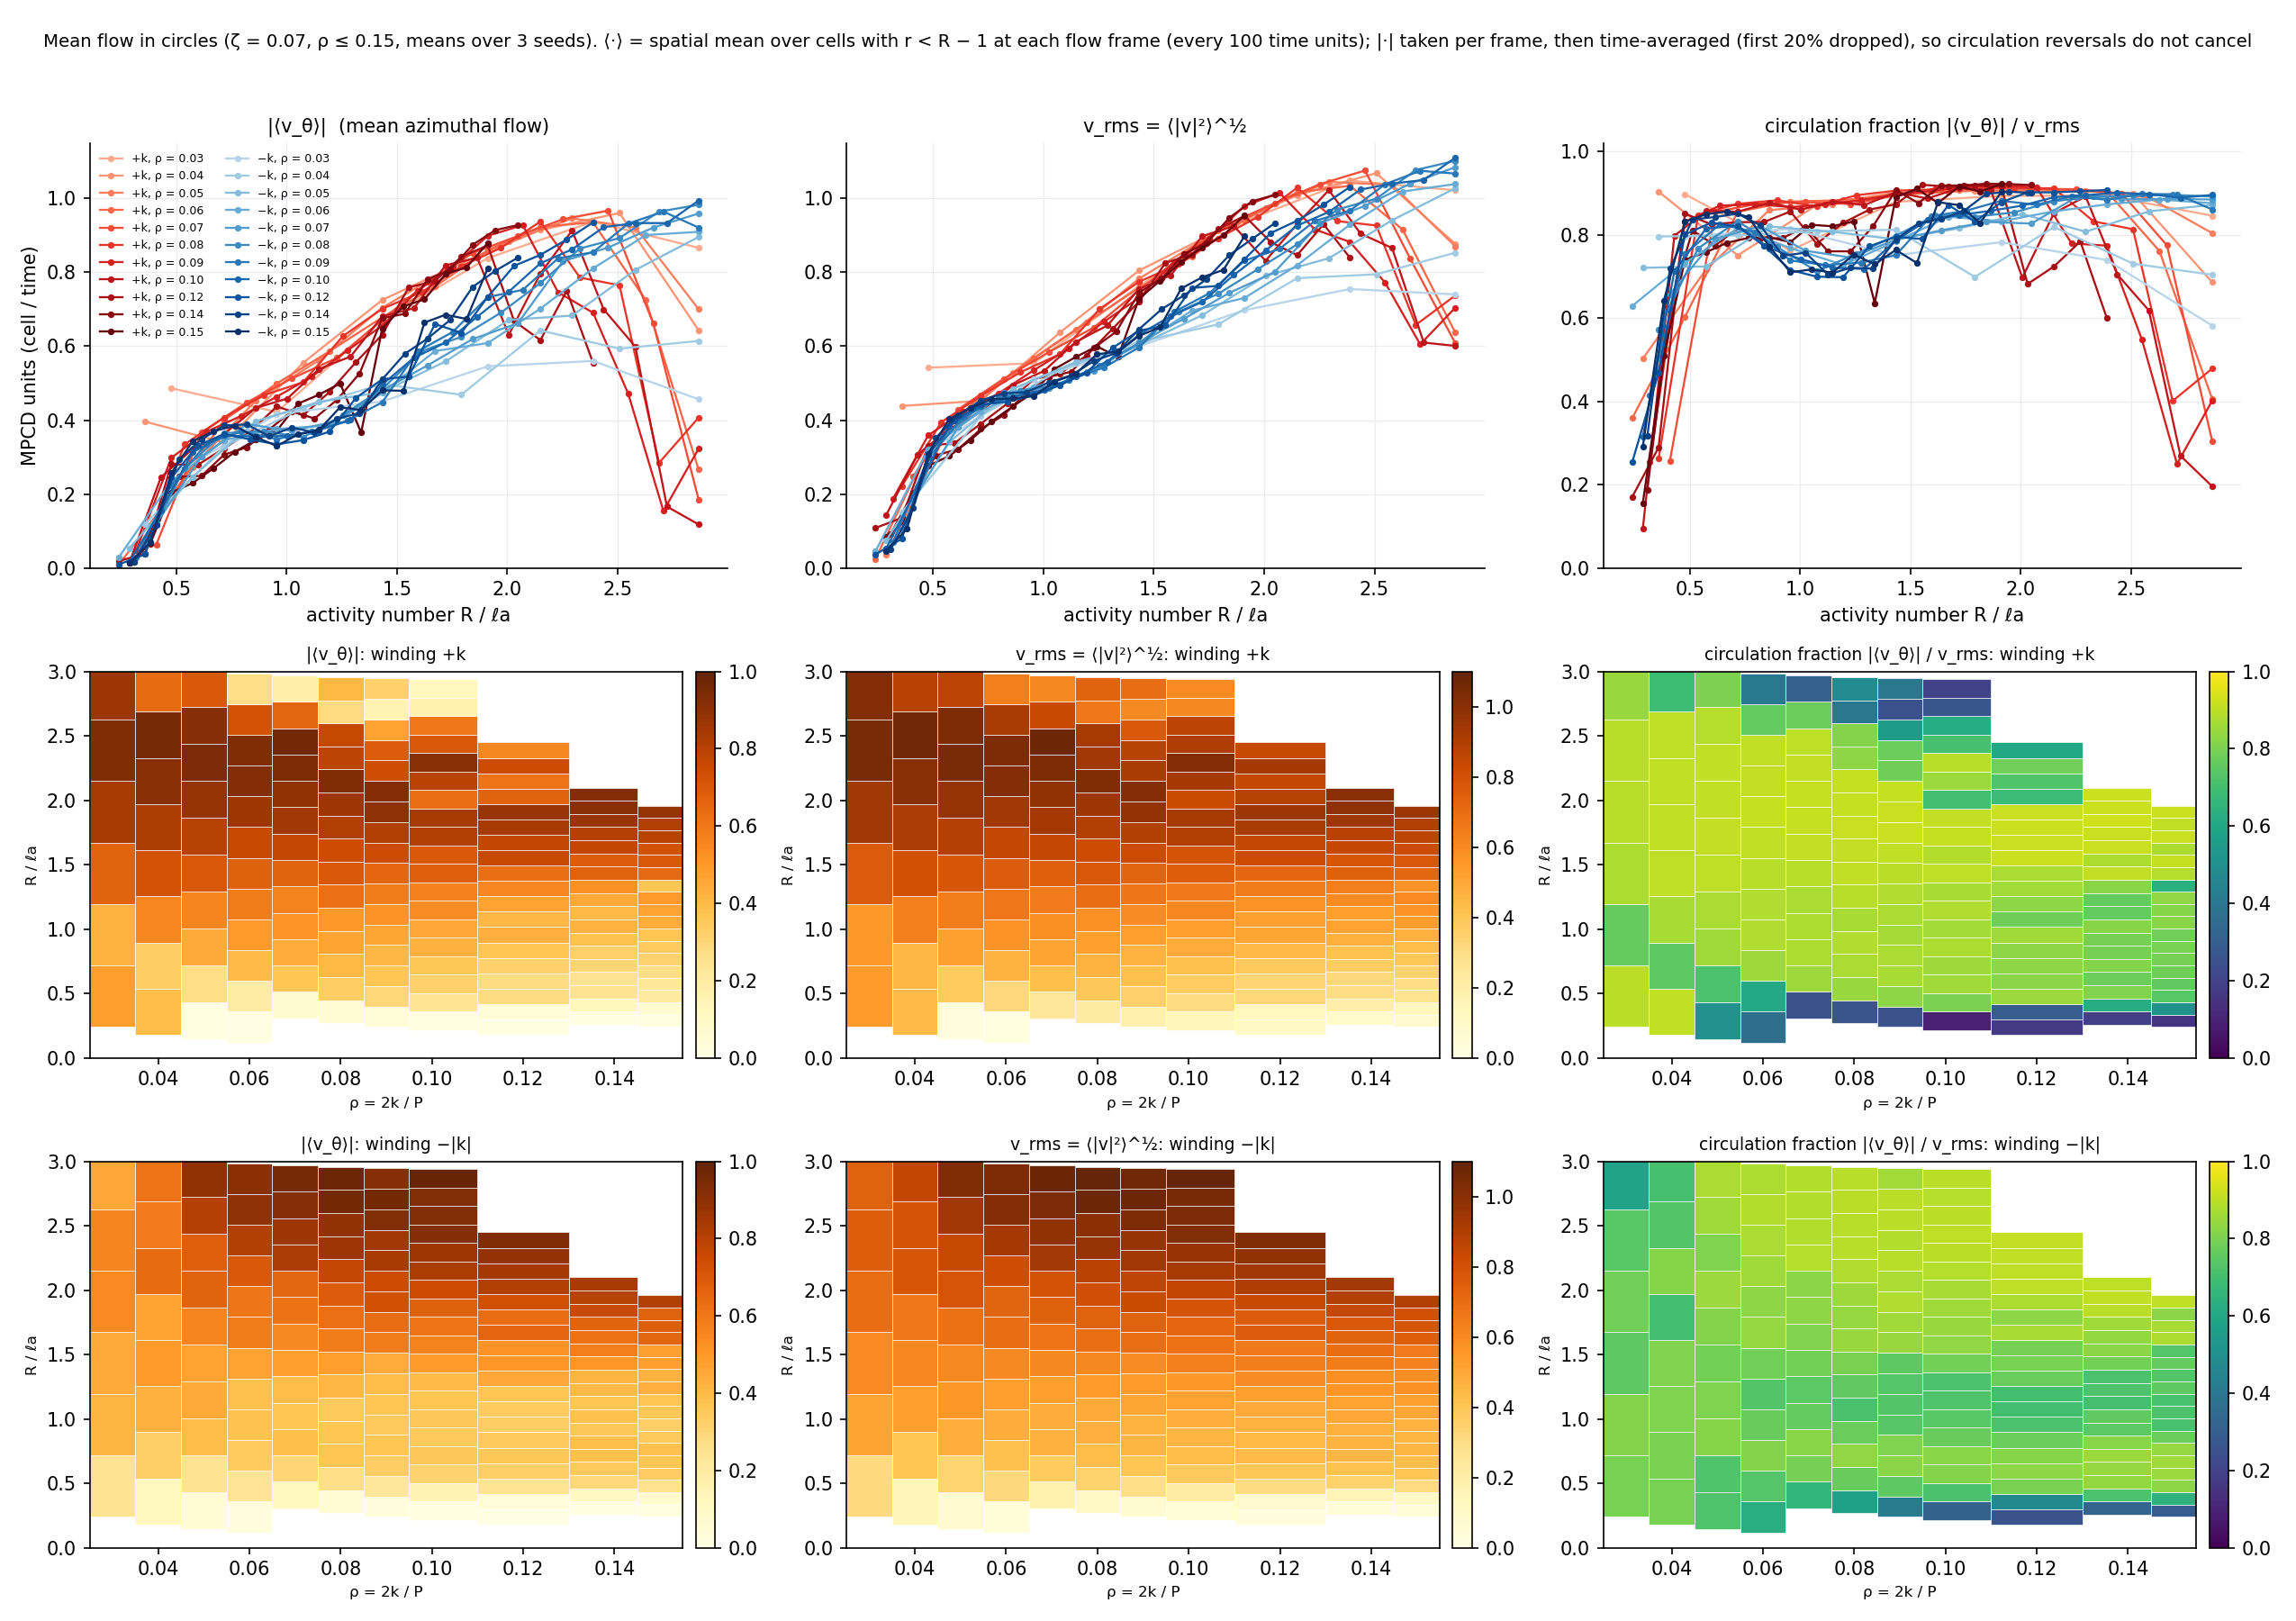
\includegraphics[width=\textwidth]{figs/flow_mean.png}\\[1ex]
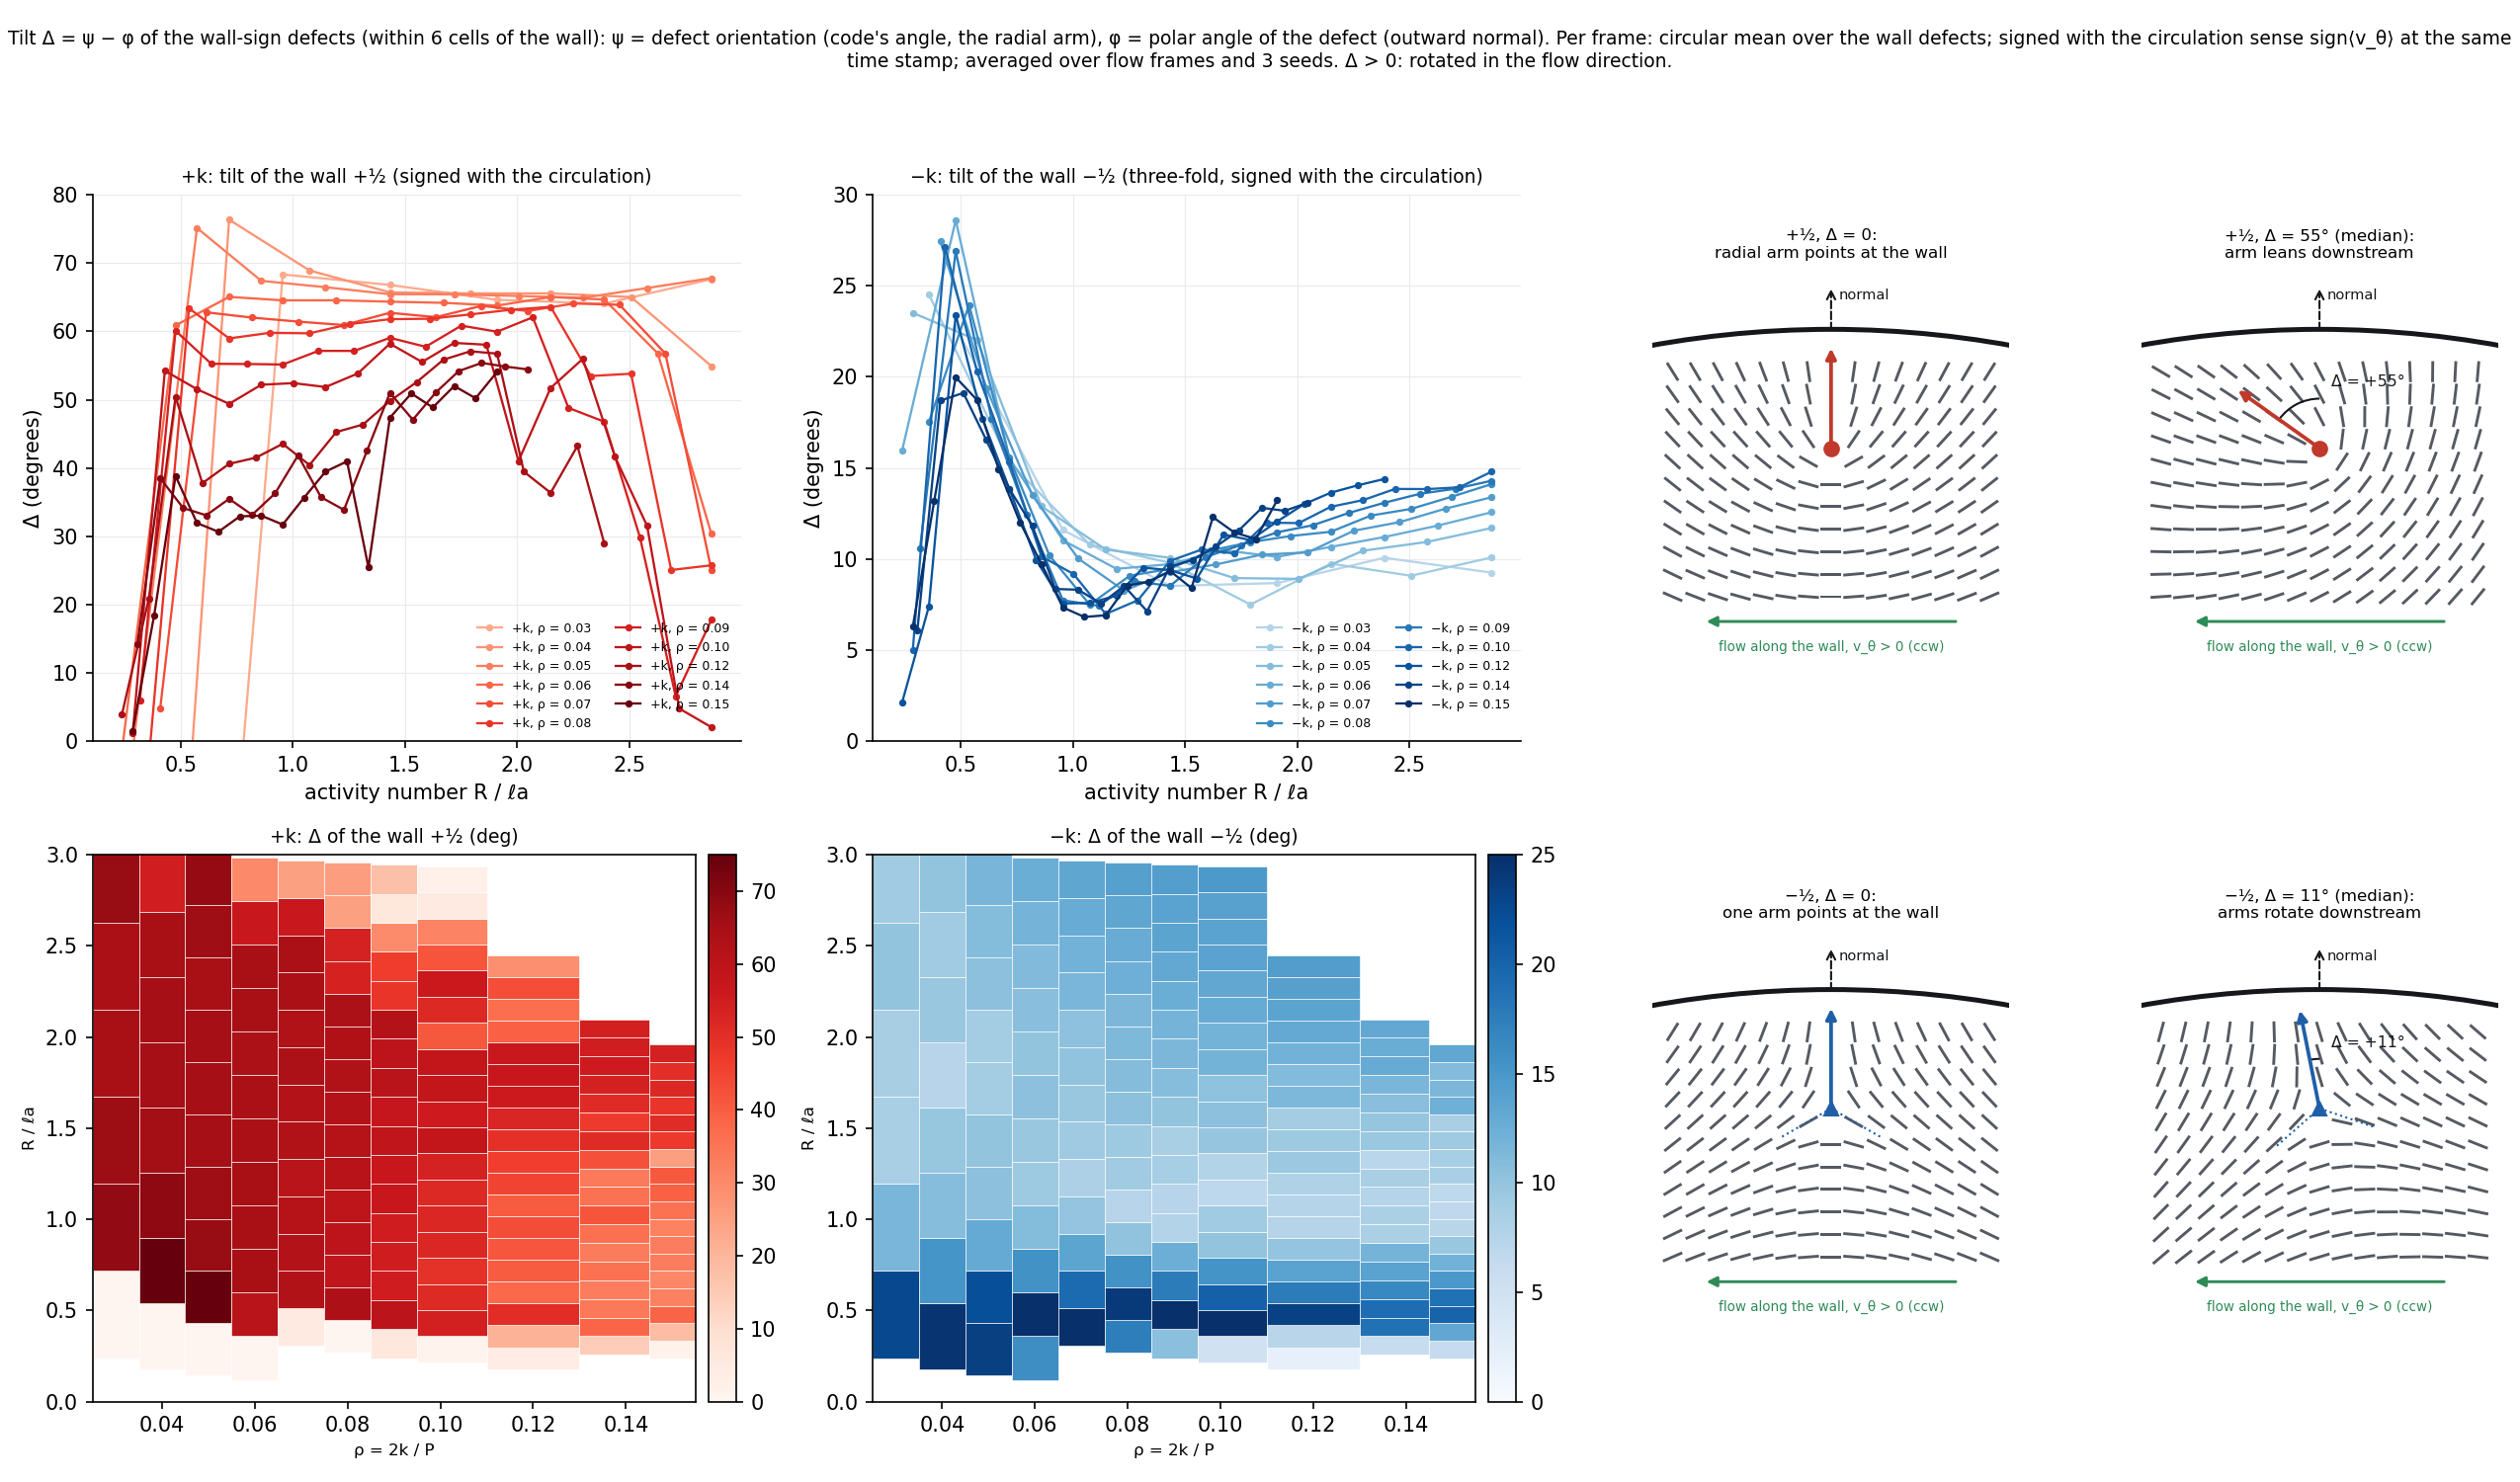
\includegraphics[width=\textwidth]{figs/flow_tilt.png}
\caption{Circles: mean flow and circulation (top) and wall-defect tilt (bottom) vs $R/\la$ and $\rho$.}\label{fig:flow}
\end{figure}

\subsection{Wall Fourier analysis for all circles}
Static and dynamic Fourier modes of the wall-sign defects along the wall (Figs.~\ref{fig:fourier-static},
\ref{fig:fourier-dyn}).
\begin{itemize}
  \item The lattice period is that of a $+1$ bulk for both windings ($2k-2$ for $+k$, $2|k|+2$ for $-k$) wherever
        $R\gtrsim0.5$--$0.75\,\la$.
  \item \textbf{Mirror runs:} the $-\tfrac12$ wall lattice has the $+1$-bulk period but is under-occupied (0.7--0.9 at low
        $\rho$, $\to1$ at high $\rho$ or large $|k|$). These vacancies are why the mirror bulk stays below $+1$; the bulk charge
        from the wall count tracks the slow-defect criterion ($r=0.96$).
  \item $+k$: full occupancy from 0.75 to $2.3\,\la$, dropping to 0.6--0.85 above $2.5\,\la$; $f_\mathrm{static}\approx0.95$--1.
  \item \textbf{No steady sliding anywhere:} lattice speed $<2$--3\% of $|\langle v_\theta\rangle|$ for $R>0.6\,\la$. The
        ``ordered but sliding'' class never appears: the layer is pinned, or vacant and melting.
\end{itemize}
\begin{figure}[h]\centering
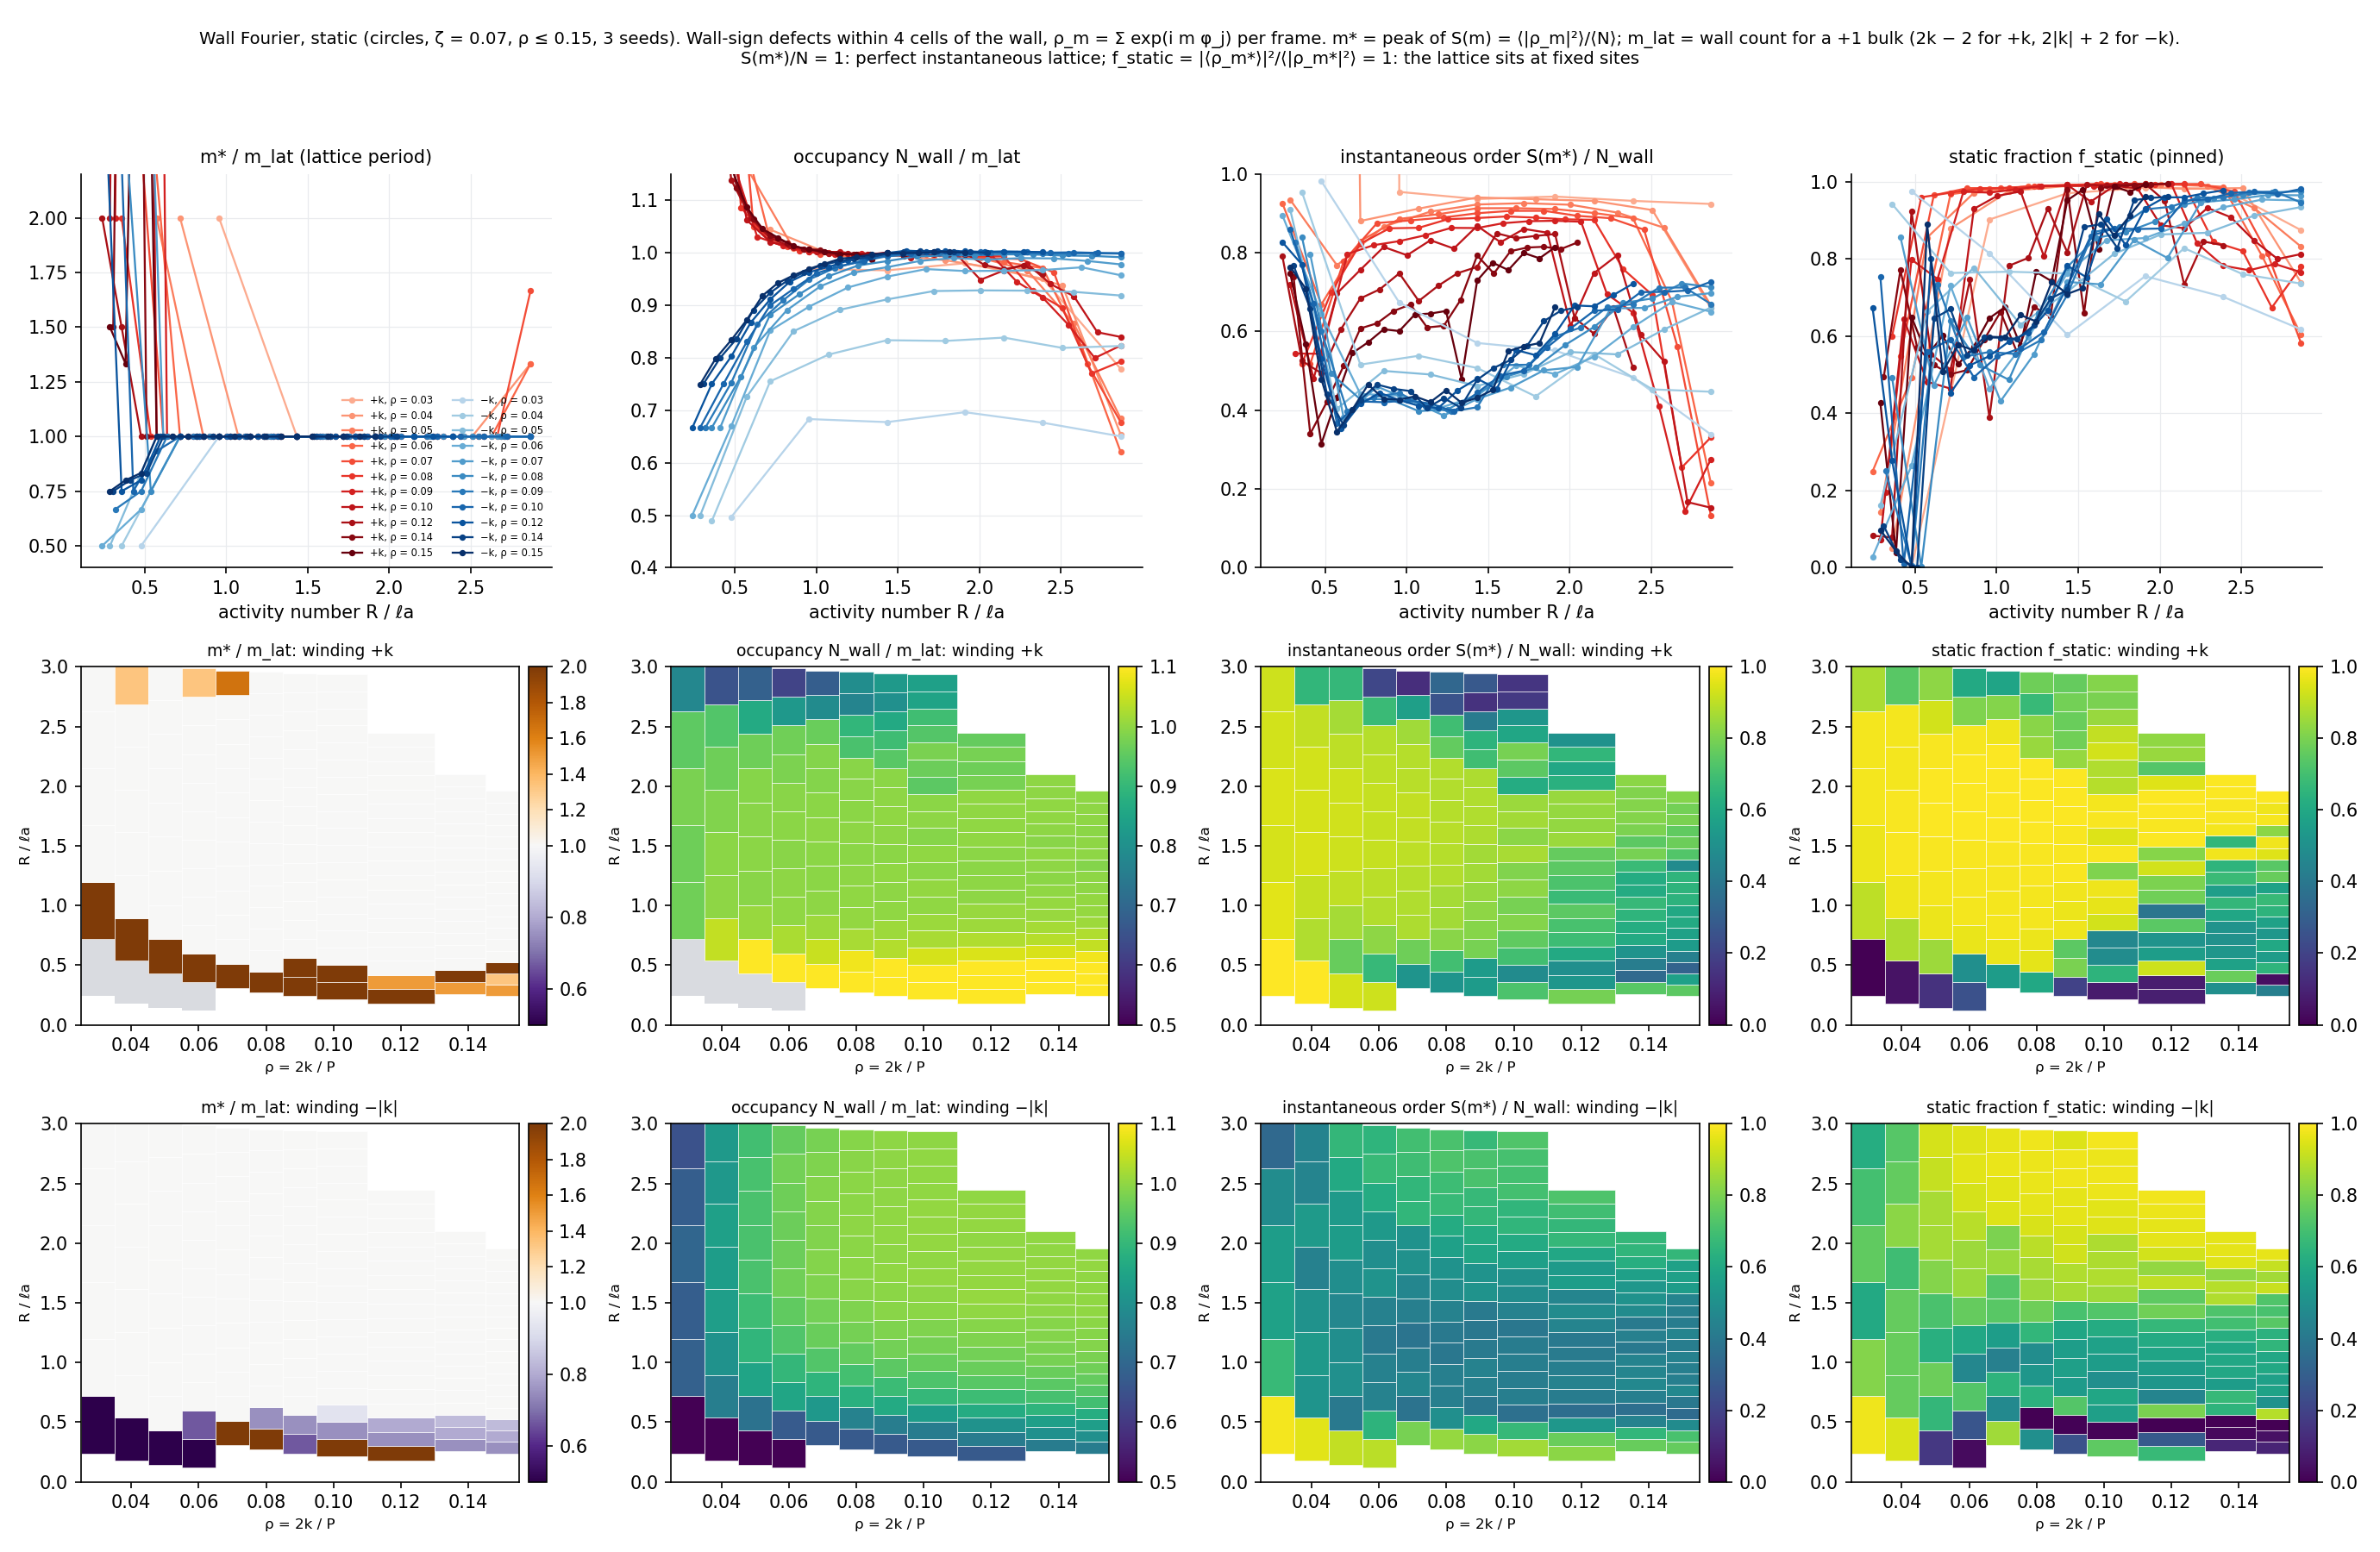
\includegraphics[width=\textwidth]{figs/fourier_static_circles.png}
\caption{Circles, static wall Fourier: lattice period, occupancy, instantaneous order and static fraction.}\label{fig:fourier-static}
\end{figure}
\begin{figure}[h]\centering
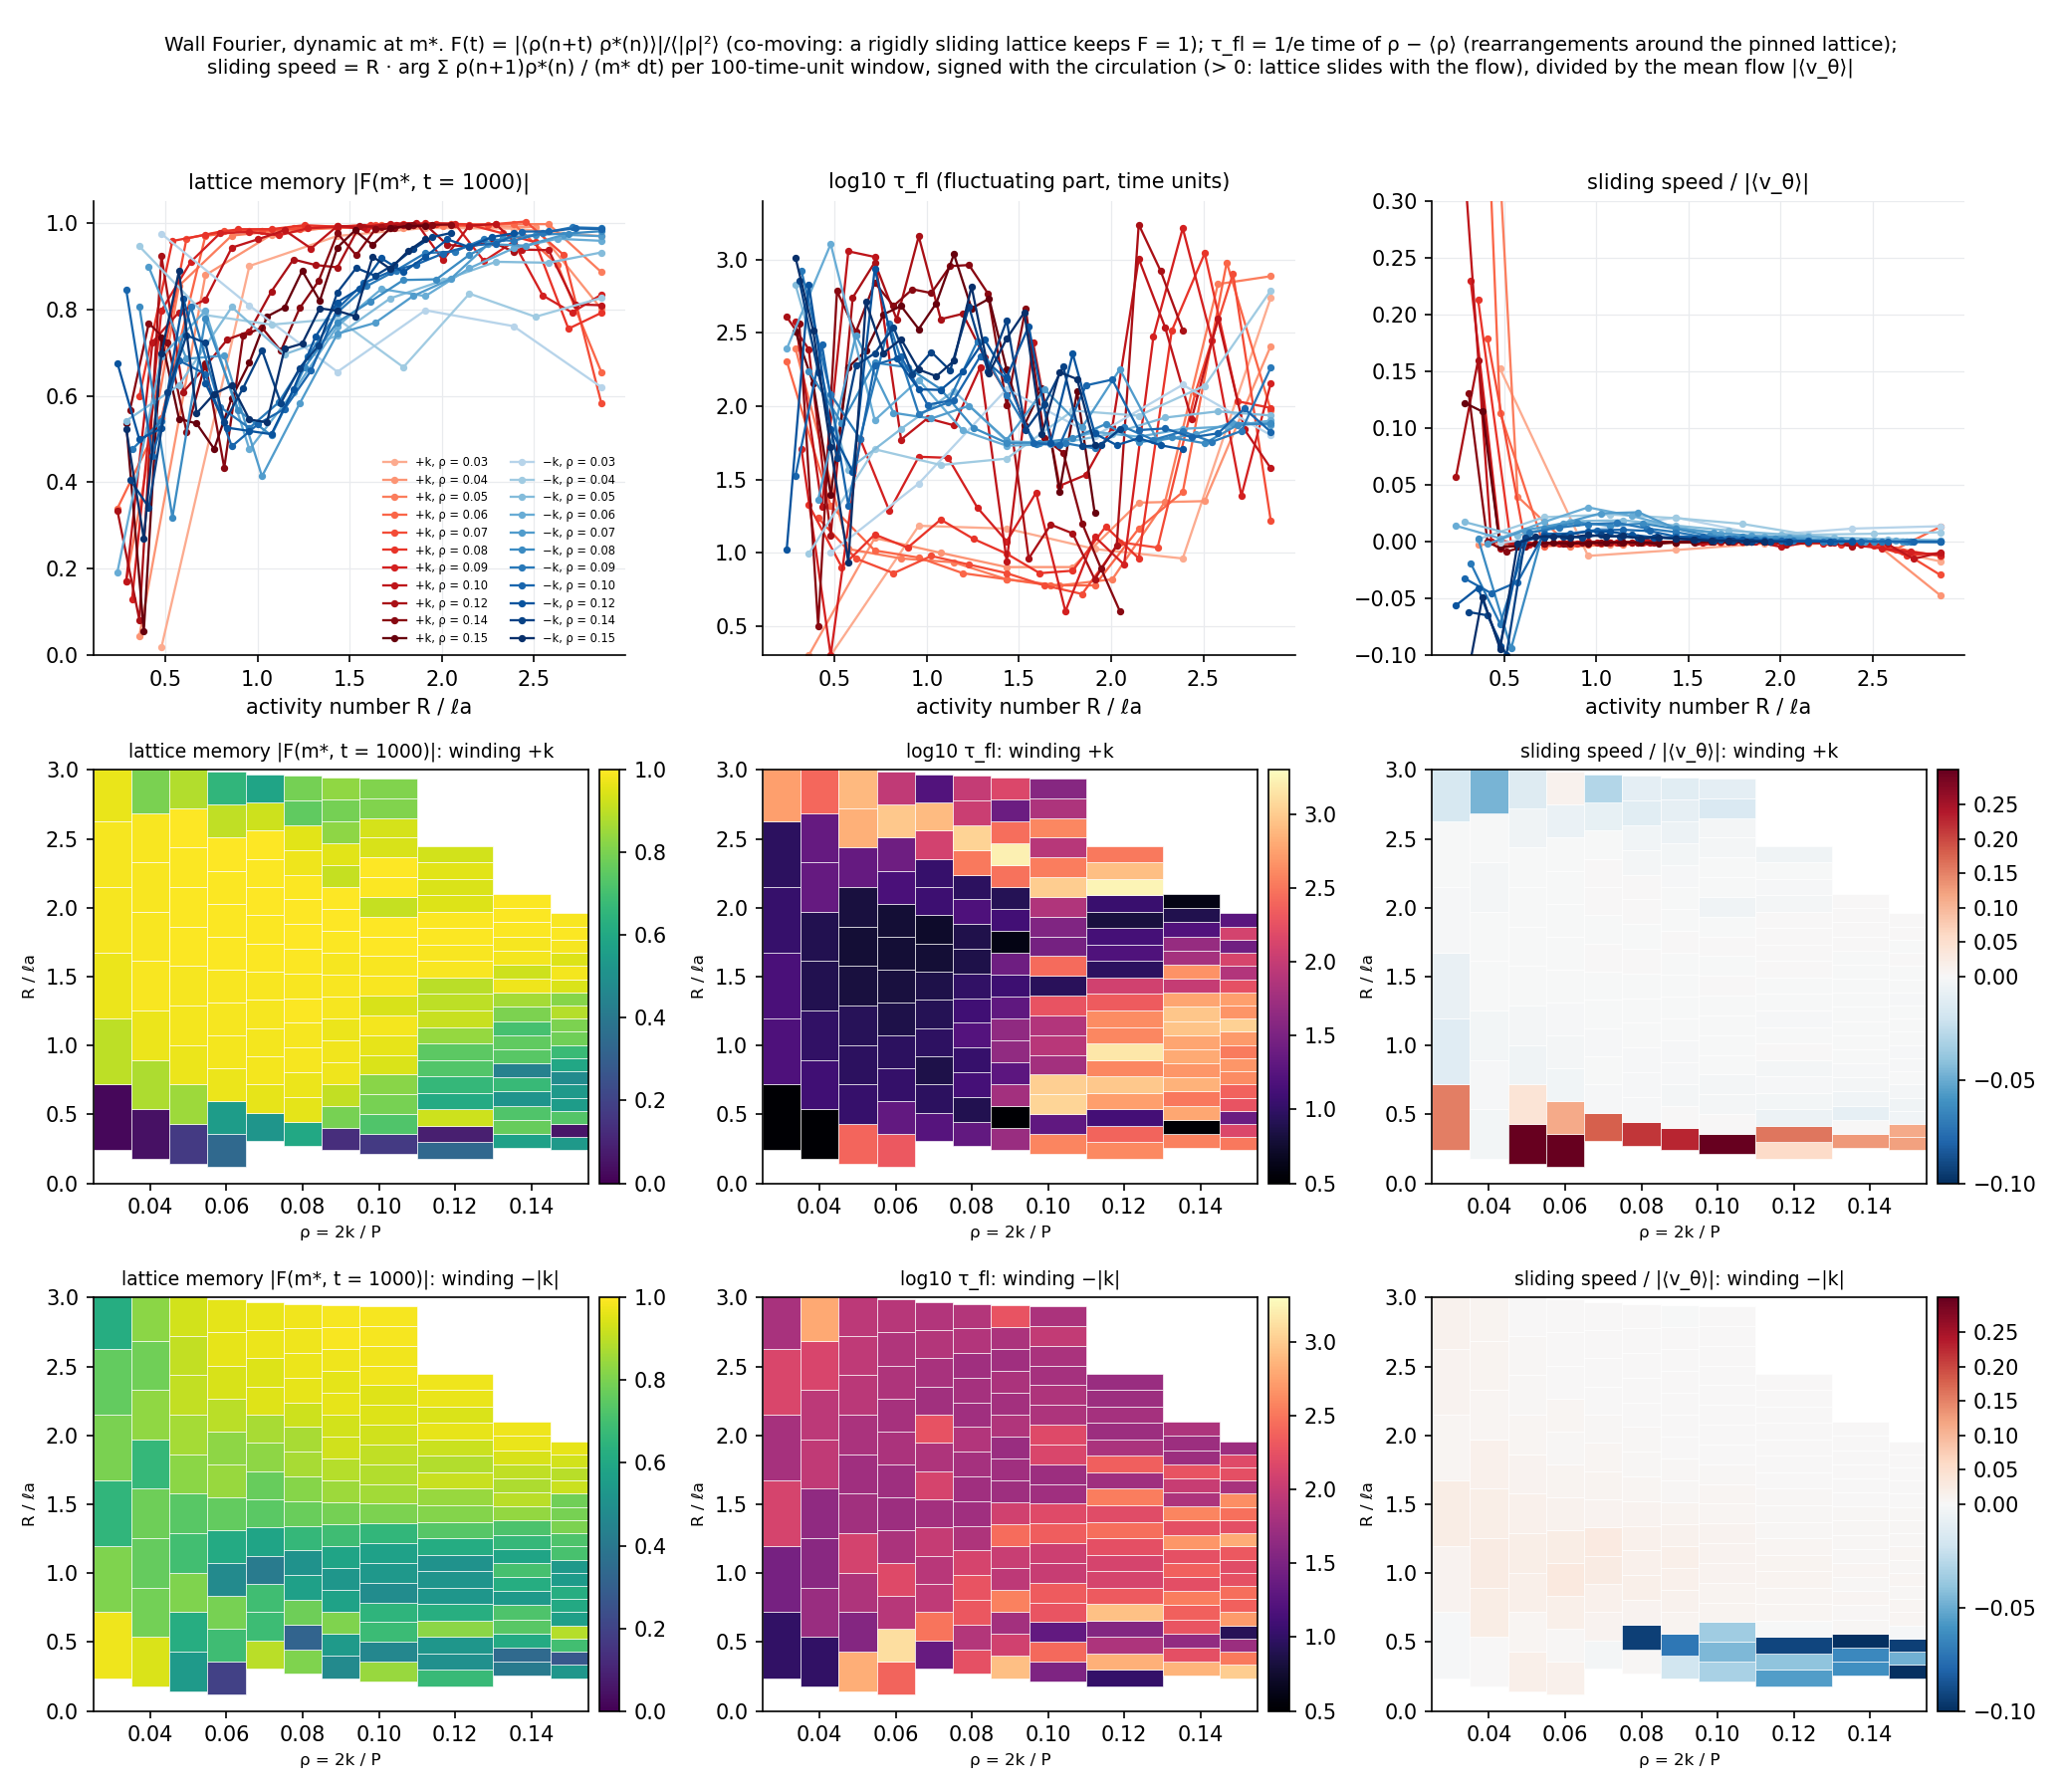
\includegraphics[width=0.85\textwidth]{figs/fourier_dynamic_circles.png}
\caption{Circles, dynamic wall Fourier: lattice memory $F(m^*,1000)$, rearrangement time and lattice sliding speed.}\label{fig:fourier-dyn}
\end{figure}

\subsection{Edge/bulk criteria over the whole sweep}
Six criteria for the bulk charge compared on 930 circle runs (Fig.~\ref{fig:criteria}).
\begin{itemize}
  \item $+k$: all criteria agree on $q_b\approx1$ for $R\approx0.8$--$2\,\la$. The knee of $Q(r)$ is the most robust
        ($\approx1$ from 0.6 to $2.4\,\la$) but undefined at large $R$ and low $\rho$. A fixed-depth cut ($r<11R/12$) fails at
        small and large $R$; density-minimum and mobility give $q_b\to0$ below $0.6$--$0.8\,\la$; slow + tilted overcounts at
        high $\rho$, where the tilt is smaller.
  \item $-|k|$: the knee value rises with $\rho$ and $R$ and reaches 0.9--1 only at $\rho\gtrsim0.10$, $R\gtrsim1.5\,\la$,
        consistent with the vacant wall lattice.
  \item For the paper: the knee as primary criterion, density minimum and mobility as cross-checks, no fixed-depth cut.
\end{itemize}
\begin{figure}[h]\centering
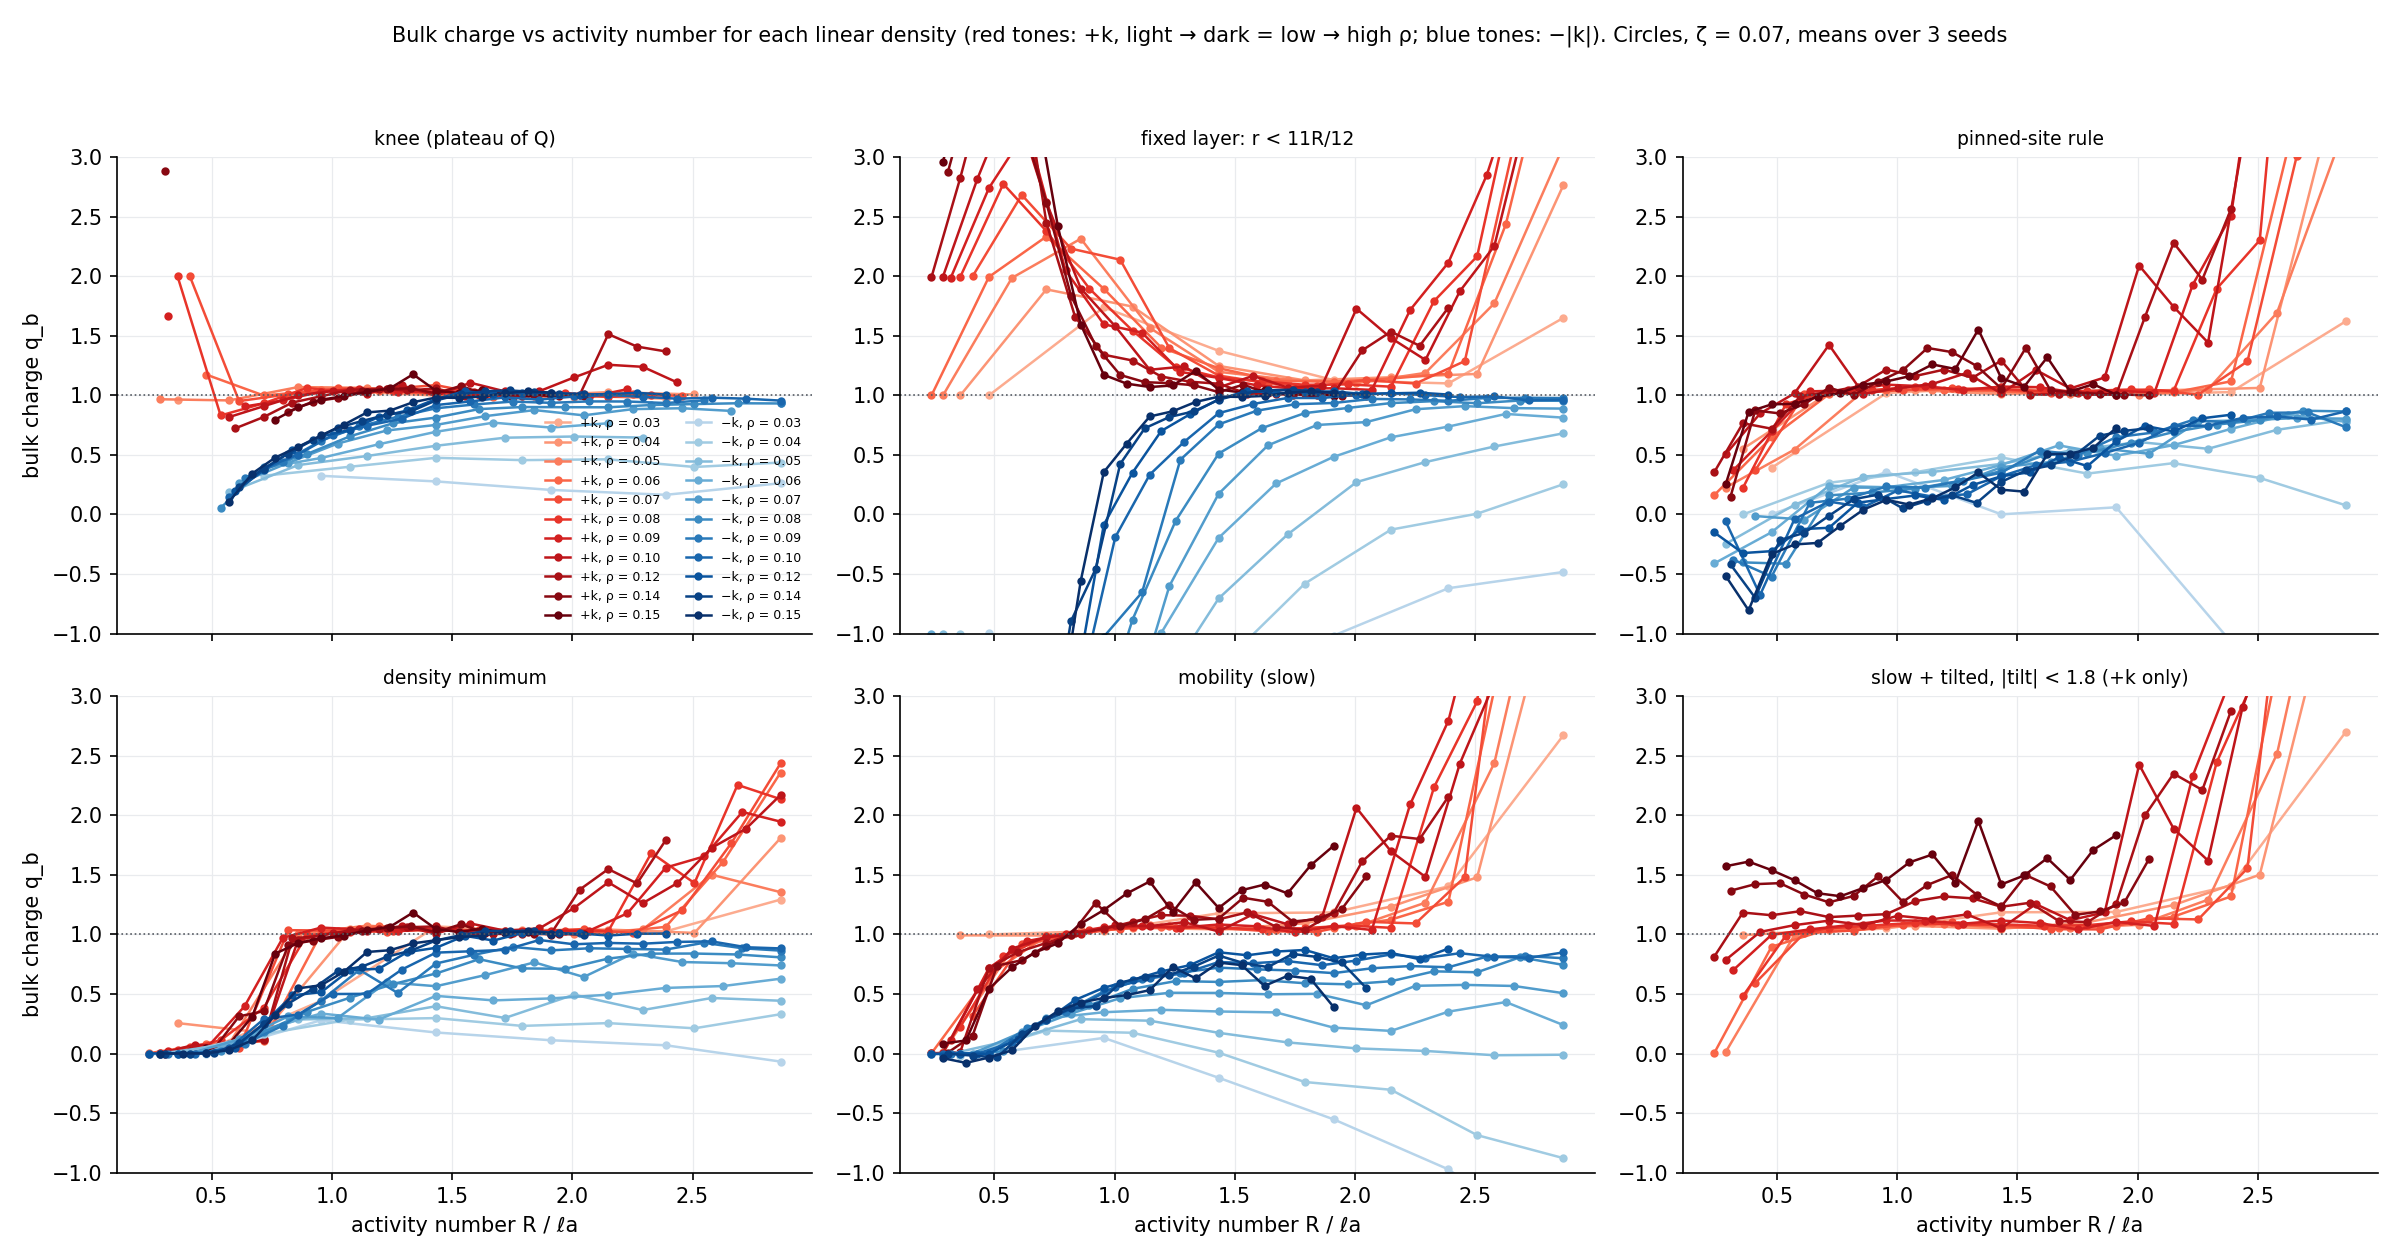
\includegraphics[width=\textwidth]{figs/criteria_bulk_vs_R.png}
\caption{Circles: bulk charge vs $R/\la$ for six edge/bulk criteria (red: $+k$, blue: $-|k|$; one curve per $\rho$).}\label{fig:criteria}
\end{figure}

\subsection{Wall dynamics in ovals and ellipses: upstream drift into vacancies}
The same analysis with positions by arclength along the real wall, for 81 oval and ellipse runs, and with a circle
reference ($k=6$, all $R$) run with the same script (Fig.~\ref{fig:walldyn}). Where the order is weak the phase of the
lattice mode is noise, so we also measure a \emph{per-defect drift}: wall $+\tfrac12$ matched between frames, $ds/dt$
along the wall, signed with the near-wall tangential flow $v_w$ (cells 1--5 from the wall).
\begin{itemize}
  \item No sliding-ordered layer in ovals either: where a lattice exists it is pinned. The near-wall flow turns with the
        bulk vortex (sign agreement 100\% with one strong vortex, 60--90\% in elongated cavities, where $|v_w|$ drops from
        0.2--0.35 to 0.03--0.07).
  \item \textbf{Wall $+\tfrac12$ drift against the wall flow, at a rate set by the vacancies of the wall lattice}, not by
        the loss of pinning: Spearman $\rho_s=-0.82$ between drift$/|v_w|$ and the vacancy fraction $1-N_\mathrm{wall}/(2k-2)$
        over all runs ($-0.93$ among pinned lattices), against $+0.18$ for $f_\mathrm{static}$. Circles ($k=6$): drift
        $\approx0$ for $R=0.7$--$1.7\,\la$, $-2\%$ at 2.15, $-18\%$ at $2.87\,\la$. The H48 $b/a=2.0$ oval is pinned
        ($f=0.84$) but 41\% empty and drifts at $-69\%$; elongated ovals $-10$ to $-80\%$.
  \item Reading: defects hop upstream into empty sites, so vacancies travel downstream. Crowded walls stop the drift:
        in the $k$ scan it vanishes from $k=6$--8 on, and in the pinched oval at $k=12$--20.
  \item Caveats: noisy for tiny circles without a vortex and for single-seed cavities; the drift includes defects entering
        or leaving the wall band.
\end{itemize}
\begin{figure}[h]\centering
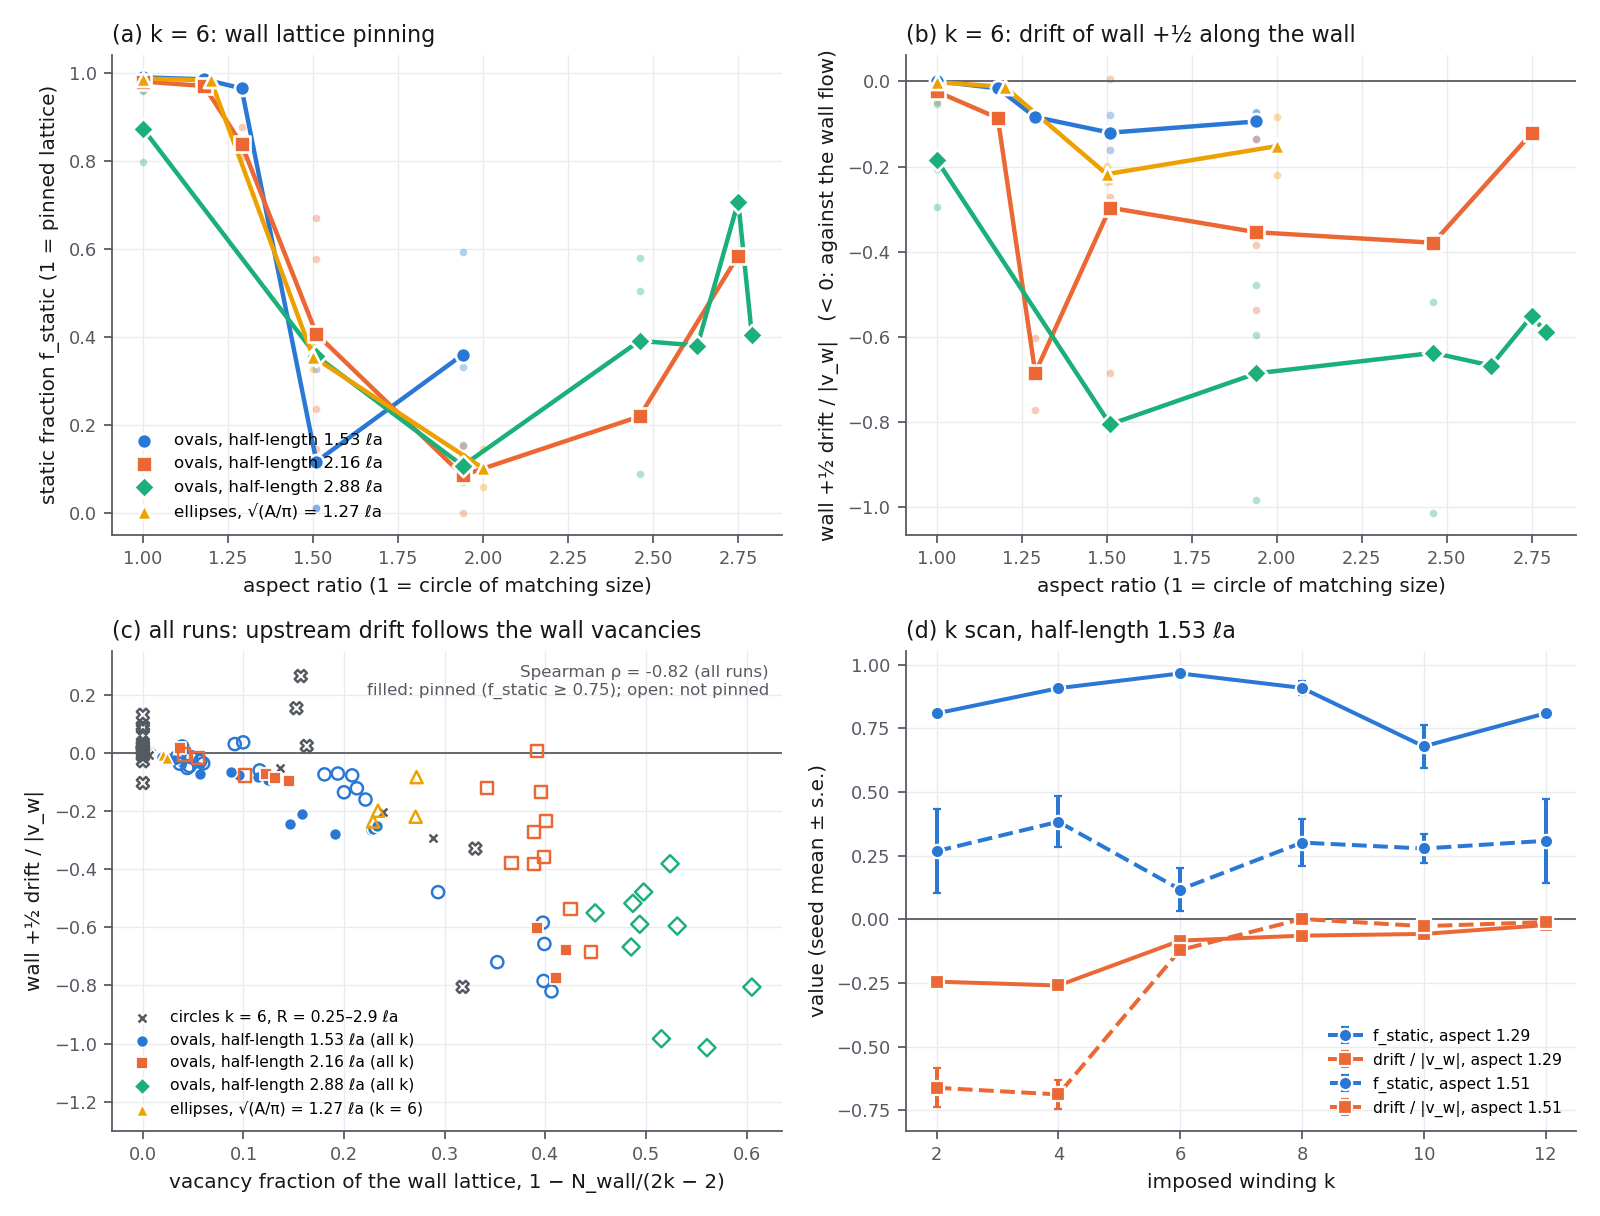
\includegraphics[width=\textwidth]{figs/wall_dynamics.png}
\caption{Ovals and ellipses vs circles. (a) static fraction vs aspect ratio ($k=6$; circles of matching size at aspect 1, in
the colour of the family they match); (b) per-defect drift$/|v_w|$; (c) drift vs vacancy fraction, all runs (filled: pinned,
$f_\mathrm{static}\ge0.75$); (d) $k$ scan at half-length $1.53\,\la$.}\label{fig:walldyn}
\end{figure}
\clearpage
